\documentclass[12pt]{report}

\usepackage{amsmath}
\usepackage{pgfplots}
\usepgfplotslibrary{units}
\usepackage[russian]{babel}
\usepackage{filecontents}
\usepackage{titlesec, blindtext, color}
\usepackage{listings}
\usepackage{pdfpages}

\usepackage{titlesec, blindtext, color} 
\definecolor{gray75}{gray}{0.75} 
\newcommand{\hsp}{\hspace{20pt}} 

\usepackage{geometry}
\geometry{top=0.5cm}

\lstset{
	language=C++,
	numbers=left,
	breaklines=true, 
	frame=single,
	texcl=true,
	basicstyle=\ttfamily,
	extendedchars=\true
}

\titleformat{\chapter}[hang]{\Huge\bfseries}{\thechapter\hsp\textcolor{gray75}{|}\hsp}{0pt}{\Huge\bfseries}

\begin{document}
	
	
	\begin{titlepage}
		\centering
		{\scshape\LARGE МГТУ им. Баумана \par}
		\vspace{3cm}
		{\scshape\Large Лабораторная работа №5\par}
		\vspace{0.5cm}	
		{\scshape\Large По курсу: "Анализ алгоритмов"\par}
		\vspace{1.5cm}
		{\huge\bfseries Конвейер\par}
		\vspace{2cm}
		\Large Работу выполнил: Подвашецкий Дмитрий, ИУ7-54Б\par
		\vspace{0.5cm}
		\LargeПреподаватели:  Волкова Л.Л., Строганов Ю.В.\par
		
		\vfill
		\large \textit {Москва, 2019} \par
	\end{titlepage}
	
	\tableofcontents
	
	\newpage
	\chapter*{Введение}
	\addcontentsline{toc}{chapter}{Введение}
	
	 При обработке данных могут возникать ситуации, когда необходимо обработать множество данных последовательно несколькими алгоритмами. В этом случае удобно использовать конвейерную обработку данных. 
	 
	 Для решения конвейреным методом была выбрана задача декодирования шифра Цезаря на основе статистического анализа.
	 
	 Всего имеется 3 ленты:
	 \begin{enumerate}
	 	\item читает сообщение;
	 	\item кодирует сообщение;
	 	\item угадывает сдвиг шифра;
	 \end{enumerate}
	 
	 \textbf{Задачами} данной лабораторной являются:
	 \begin{enumerate}
	 	\item изучение метода конвеерной обработки данных;
	 	\item реализация данного метода;
	 	\item экспериментальное подтверждение работостопобности алгоритма;
	 \end{enumerate}

	\chapter{Аналитическая часть}
	
	\section{Описание алгоритма}
	
	Сначала запускается 3 параллельных процесса, каждый из которых отвечает за определенную ленту. Каждому процессу присвоена своя очеред заданий. Процесс проверяет есть ли в очереди задания, если есть, то забирает его из очереди, обрабатывает и отправляет в следующую очередь, иначе ждет поступления задания.
	
	После того как 3 ленты запустились, запускается параллельный процесс, отвечающий за генерацию заданий. Этот процесс создает задания и помещает их в первую очередь, тем самым запуская обработку.
	
	Завершение каждой из трех конвейерных лент происходит в том случае, если время ожидания задания, в некоторый момент времени, превосходит удвоенное среднее время ожидание на этой ленте. Среднее время ожидания высчитывается по мере работы алгоритма.
	
	Первая лента реализует чтение сообщения. Необходимо, чтобы в задании было указано имя файла, в котором находится сообщение.
	
	Вторая лента реализует шифрование шифром Цезаря.[2]
	
	Третья лента подсчитывает частоту встречи каждой буквы в сообщении, и сверяет со статистическими данными. [1]
	На основе сравнение выдвигается предположение о изначальном сдвиге шифрованного сообщения.


	\section*{Вывод}
	\addcontentsline{toc}{chapter}{Вывод}

	В данном разделе была описана схема работы конвейера и реализуемая задача.

	\chapter{Конструкторская часть}

	\section{Схема алгоритмов}
	
	\subsection{Схема работы ленты}
	
	Так как все 3 ленты однотипны, далее будет описан общий принцип работы каждой ленты.
	
	\begin{center}
		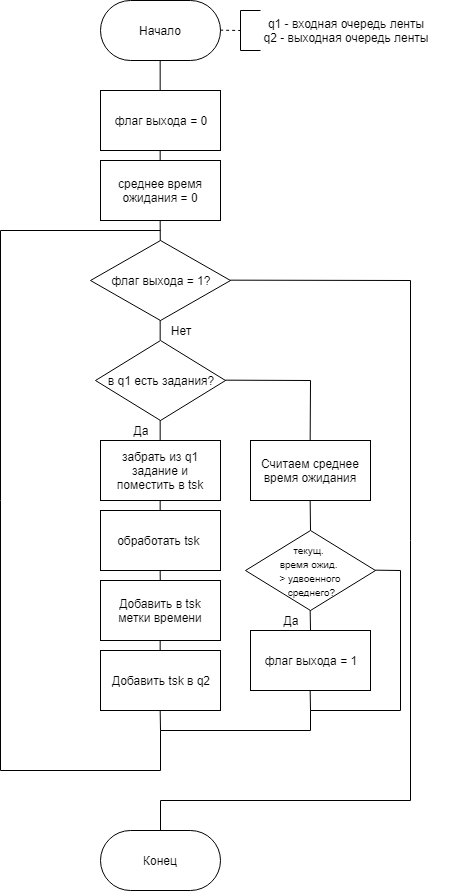
\includegraphics[scale=0.5]{tape.png}
		
		Рис.1. Схема работы ленты
	\end{center}

	\section*{Вывод}
	\addcontentsline{toc}{chapter}{Вывод}
	
	В данном разделе была разработана схема работы ленты.
	
	\chapter{Технологическая часть}
	
	\section{Выбор ЯП}
	В качестве языка программирования был выбрал C++, так как он позволяет реализовать задачу максимально эффективно.
	
	\section{Замеры времени}
	Замер времени работы алгоритмов производился при помощи функций из библиотеки <chorno>.[3] Для реализации потоков была выбрана библиотека <thread>.[4] Для реализации раздленного доступа к ресурсам использовалась библиотека <mutex>.[5]
	
	\section{Требования к ПО}
	
	\textbf{Требования к выводу:}
	\begin{enumerate}
		\item информация о временных метках каждого задания;
	\end{enumerate}
	\textbf{Требования к программе:}
	\begin{enumerate}
		\item Корректный вывод, программа не должна аварийно завершаться
	\end{enumerate}
	
	\textbf{Требования структуре входного файла:}
	В считываемом файле должны быть буквы Анлгийского алфавита. Так же допуситимы знаки пробела, запятой и точки.
	
	\section{Сведения о модулях программы}
	Программа состоит из:
	\begin{itemize}
		\item main.cpp - главный файл программы
		\item conveyor.cpp - файл с реализацией конвейера(Листинг 3.1.)
	\end{itemize}
	
	\section{Листинг кода}
	
	Листинг 3.1. Реализация конвейера.
	\lstinputlisting[language=C++]{../lab_05/conveyor.cpp}
	
	\section*{Вывод}
	\addcontentsline{toc}{chapter}{Вывод}
	
	В данном разделе были реализованных необходимые алгоритмы.
	
	\chapter{Экспериментальная часть}
	
	\section{Постановка эксперимента}

	Создадим 5 заданий и посмотрим временные метки от каждой ленты.
	
	\section{Пример работы}
	
	На рисунке ниже представлены временные метки каждого обработанного задания.
	\begin{enumerate}
	\item Task Id: N - номер задания
	\item N tape st/end - время начала/конца обработки на N ленте
	\item encoden num - сдвиг при кодировке
	\item deconded num - предпологаемый сдвиг
	\end{enumerate}

	\begin{center}
		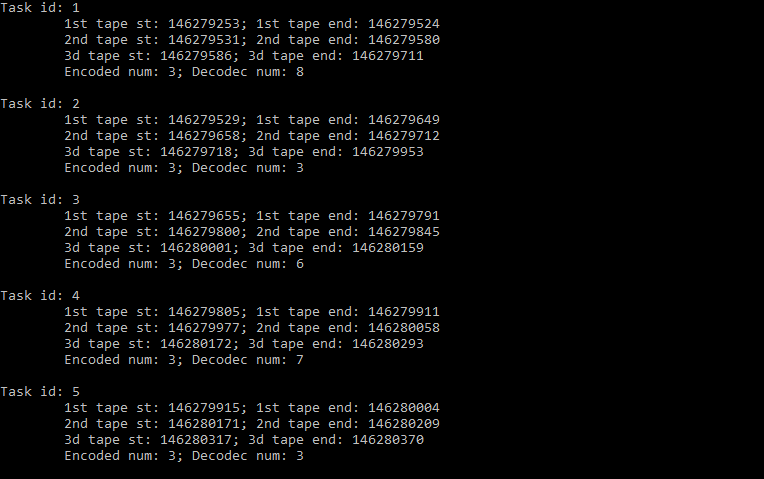
\includegraphics[scale=0.8]{exp.png}
		
		Рис. 2. Временные метки обработанных заданий.
	\end{center}

	\section*{Вывод}
	\addcontentsline{toc}{chapter}{Вывод}
	
	На основе приведенных выше (Рис. 2.) временных меток обрабоки каждого задания, можно сделать вывод что конвейер работает правильно, т.е. время начала обработки всегда меньше времени конца, и так же видно как после выхода задания с ленты, на эту ленту поступает другое задание.
	
	Задание 1 поступило на первую ленту в 146279253 мкс, вышло в 146279524 мкс.
	Задание 1 поступило на вторую ленту в 146279531 мкс, в тоже время Задание 2 поступило на первую ленту в 146279529.
	
	Так же можно заметить, что данный алгоритм угадывает зашифрованное сообщение в 2 из 5 случаев, что не является хорошим результатом.
	Для улучшения этого результата можно увеличить объем изходного текста, так как алгоритм завязан на статичтическом анализе.
	
	\chapter*{Заключение}
	\addcontentsline{toc}{chapter}{Заключение}
	
	В результате данной лабораторной работы было:
	\begin{enumerate}
		\item изучен метод конвейерной обработки данных;
		\item реализован данный метод;
		\item эксперементально подтверждено корректная работа алгоритма (Рис. 2.);
	\end{enumerate}

	На Рис. 2. можно увидеть, что Задание 1 поступило на первую ленту в 146279253 мкс, вышло в 146279524 мкс.
	Задание 1 поступило на вторую ленту в 146279531 мкс, в тоже время Задание 2 поступило на первую ленту в 146279529.

\chapter*{Список литературы}
\addcontentsline{toc}{chapter}{Список литературы}
\begin{enumerate}
	\item Основы криптоанализа. [Электронный ресурс] Режим доступа: http://www.univer.omsk.su/omsk-old/Edu/infpro/1/kodir/kripan.html 
	Последння дата обращения: 17.12.2019
	\item Шифр Цезаря. [Электронный ресурс] 
	Режим доступа: http://kriptografea.narod.ru/chezar.html Последння дата обращения: 17.12.2019
	\item <chrono>. [Электронный ресурс] 
	Режим доступа: http://www.cplusplus.com/reference/chrono/ Последння дата обращения: 17.12.2019
	\item std::thread. [Электронный ресурс] 
	Режим доступа: https://ru.cppreference.com/w/cpp/thread/thread Последння дата обращения: 17.12.2019
	\item std::mutex. [Электронный ресурс] 
	Режим доступа: https://ru.cppreference.com/w/cpp/thread/mutex Последння дата обращения: 17.12.2019
\end{enumerate}


\end{document}



